\documentclass[12pt,openany]{report}
\title{Eigenmath Manual}
\author{George Weigt}
\date{April 4, 2007}
\pagestyle{headings}
\usepackage{graphicx}

%\parindent=0.3in

\begin{document}
\maketitle
\tableofcontents

\newpage

\chapter{The Big Picture}
In simplest terms, when you type something into Eigenmath,
it gets evaluated and the result is printed.
For a first example, try entering $1/2+1/3$.

\medskip
{\tt 1/2+1/3}

$$5\over6$$

\medskip
\noindent
As you can see, Eigenmath uses rational arithmetic for numerical calculations.
You can enter ``float'' to convert the result to a floating point number.

\medskip
{\tt float}

$$0.833333$$

\medskip
\noindent
There are a number of features for doing symbolic calculations.
Here is a preview.

\medskip
{\tt integral(log(x))}

$$-x+x\log(x)$$

\newpage

\noindent
Here is a simple example that draws the graph of $y=mx+b$.

\medskip
{\tt y=m*x+b}

{\tt m=1/2}

{\tt b=-3}

{\tt draw(y)}

\medskip
\noindent
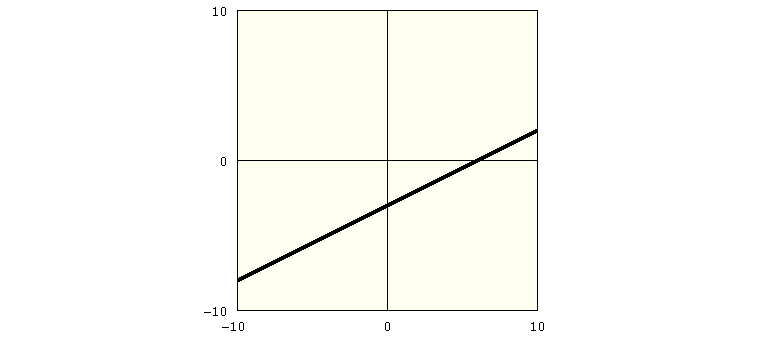
\includegraphics[scale=0.5]{1.png}

\newpage

\noindent
Now suppose that we want to draw a graph
using different values for $m$ and $b$.
We could type in everything all over again, but it would be easier
in the long run to write a script.
Then we can go back and quickly change $m$ and $b$ as many times as we want.

\medskip
\noindent
To prepare a script, click on the Edit Script button.
Then enter the script commands, one per line.

\medskip
{\tt y=m*x+b}

{\tt m=1/2}

{\tt b=-3}

{\tt draw(y)}

\medskip
\noindent
Next, click on the Run Script button to see the graph.

\medskip
\noindent
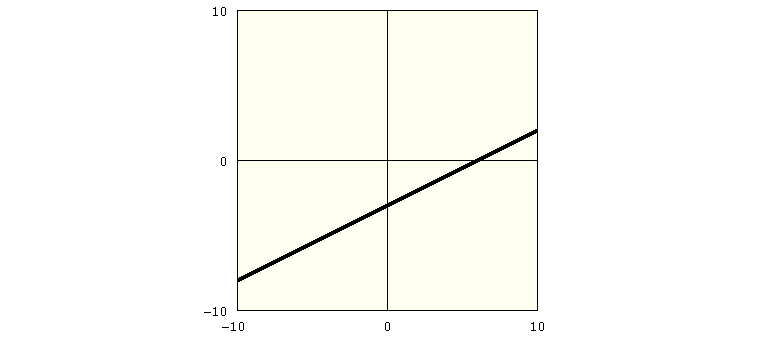
\includegraphics[scale=0.5]{1.png}

\medskip
\noindent
Eigenmath runs a script by stepping through it line by line.
Each line is evaluated just like a regular command.
This continues until the end of the script is reached.
After the script runs, you can click Edit Script and go back and change something.

\newpage

\noindent
You may have noticed that when we define a symbol
like $y=mx+b$, no result is printed.
Eigenmath works this way so the screen does not get cluttered
up with intermediate results.
When you want to see the value of a symbol, just enter it.

\medskip
{\tt y}
$$y=mx+b$$

\medskip
\noindent
Symbols can also be defined as functions of one or more variables.
In the following example, we define $y$ as a function of $x$.
Just like before, we can enter $y$ to see its value and
also draw $y$.
The main difference is that now we can easily evaluate $y$ for
a specific value of $x$.

\medskip
{\tt y(x)=m*x+b}\par
{\tt y}
$$y=mx+b$$\par
{\tt y(0)}
$$-3$$

\medskip
\noindent
Here is an example of a function of two variables.

\medskip
{\tt r(x,y)=(x{\char94}2+y{\char94}2){\char94}(1/2)}\par
{\tt r}
$$r=(x^2+y^2)^{1/2}$$
\indent
{\tt r(1,2)}
$$5^{1/2}$$

\medskip
\noindent
We are now ready to move on so
it is time to clear out the old definitions
with the following command.

\medskip
{\tt clear}

\medskip
\noindent
Clicking on the Clear button does the same thing.
It should also be pointed out that Eigenmath automatically does a clear before
running a script.

\newpage

\chapter{Linear Algebra}

\newpage

\noindent
Vectors and matrices are entered like this.

\medskip
{\tt X=(x1,x2,x3,x4)}

{\tt A=((1,2,3),(4,5,6),(7,8,9))}

{\tt A}

$$\left(\matrix{1&2&3\cr4&5&6\cr7&8&9\cr}\right)$$

\medskip
\noindent
Eigenmath's dot function is used to multiply vectors and matrices.
The following example shows how to use dot and inv to solve for $\bf X$ in $\bf AX=B$.

\medskip
{\tt A=((3.8,7.2),(1.3,-0.9))}

{\tt B=(16.5,-22.1)}

{\tt X=dot(inv(A),B)}

{\tt X}

$$\left(\matrix{-11.2887\cr8.24961}\right)$$

\medskip
\noindent
Individual tensor components can be accessed using square brackets.
Index numbering begins with 1.

\medskip
{\tt A=zero(2,2)}

{\tt A[1,2]=a}

{\tt A}

$$\left(\matrix{0&a\cr0&0\cr}\right)$$

\newpage

\chapter{Draw}

\newpage

\noindent
draw($f,x$) draws a graph of the function $f$ of $x$.
The second argument can be omitted when the dependent variable
is literally $x$ or $t$.
The vectors $xrange$ and $yrange$ control the scale of the graph.

\medskip
{\tt draw(x{\char94}2)}

\medskip
\noindent
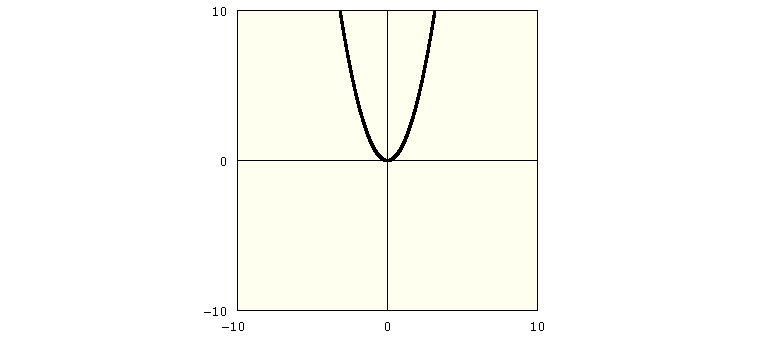
\includegraphics[scale=0.5]{parabola.png}

{\tt xrange=(-1,1)}

{\tt yrange=(0,2)}

{\tt draw(x{\char94}2)}

\medskip
\noindent
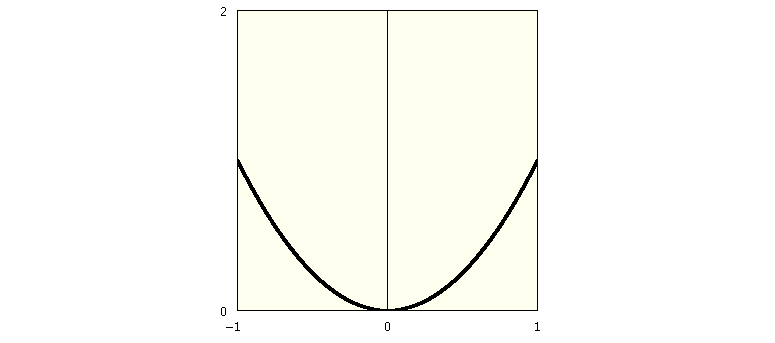
\includegraphics[scale=0.5]{parabola2.png}

{\tt clear}

\medskip
\noindent
The clear command (or a click of the Clear button)
resets $xrange$ and $yrange$.

\newpage

\noindent
Parametric drawing occurs when a function returns a vector.
The vector $trange$ controls the parameter range.
The default range is $(-\pi,\pi)$.

\medskip
{\tt f=(cos(t),sin(t))}

{\tt draw(5*f)}

\medskip
\noindent
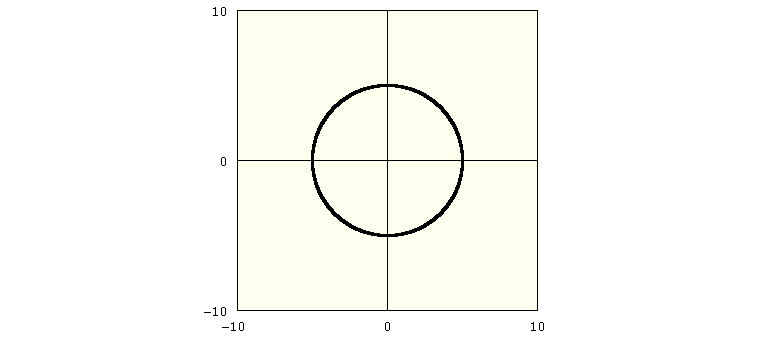
\includegraphics[scale=0.5]{circle.png}

{\tt trange=(0,pi/2)}

{\tt draw(5*f)}

\medskip
\noindent
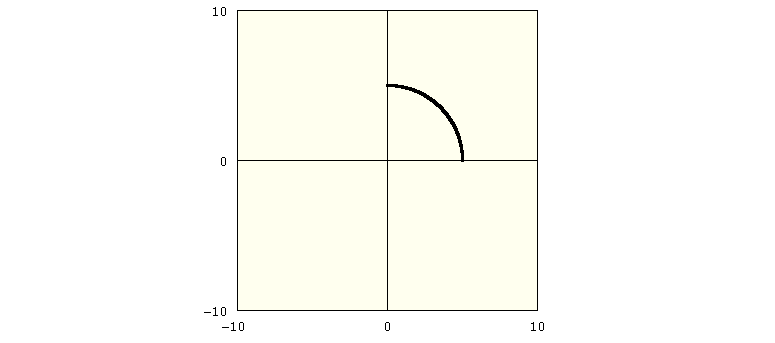
\includegraphics[scale=0.5]{circle2.png}

{\tt clear}

\chapter{Calculus}

\label{d}

The function d($f,x$) returns the derivative of $f$ with respect to $x$.
The $x$ can be omitted for expressions in $x$.

\medskip
{\tt d(x{\char94}2)}

$$2x$$

\medskip
\noindent
Multi-derivatives can be obtained by extending the argument list.

\medskip
{\tt r=sqrt(x{\char94}2+y{\char94}2)}

{\tt d(r,x,y)}

$${-{xy\over(x^2+y^2)^{3/2}}}$$

\medskip
\noindent
A gradient can be obtained by using a vector for the second argument.

\medskip
{\tt r=sqrt(x{\char94}2+y{\char94}2)}

{\tt d(r,(x,y))}

$$\left(\matrix{
\displaystyle{{x\over(x^2+y^2)^{1/2}}}\cr
\cr
\displaystyle{{y\over(x^2+y^2)^{1/2}}}\cr
}\right)$$

\newpage

\noindent
Here is a trick.
The function $f$ in d($f$) does not have to be defined.
Eigenmath will check the argument list
of $f$ to figure out what to do.

\medskip
{\tt d(f(x),(x,y))}

$$\left(\matrix{
\partial(f(x),x)\cr
\cr
0\cr
}\right)$$

{\tt d(f(),(x,y))}

$$\left(\matrix{
\partial(f(),x)\cr
\cr
\partial(f(),y)\cr
}\right)$$

\medskip
\noindent
As the second example shows,
if the argument list is empty then $f$ is assumed to depend
on any variable that d encounters.

\medskip
\noindent
This ``generic'' function property is useful for experimenting with
differential forms.
For example, let us check the following identity.
$$\mathop{\rm div}(\mathop{\rm curl}{\bf F})=0$$

\medskip
{\tt curl(F)=(d(F[3],y)-d(F[2],z),d(F[1],z)-d(F[3],x),d(F[2],x)-d(F[1],y))}

{\tt div(F)=d(F[1],x)+d(F[2],y)+d(F[3],z)}

{\tt F=(FX(),FY(),FZ())}

{\tt div(curl(F))}

$$0$$

\medskip
\noindent
Pleas see page \pageref{curl-example} for another example.

\newpage

\label{integral}

\noindent
Let us move on now to integrals.

\medskip
\noindent
The function integral($f,x$) returns the integral of $f$ with respect to $x$.
The $x$ can be omitted for expressions in $x$.
A multi-integral can be obtained by extending the argument list.

\medskip
{\tt integral(x{\char94}2)}

$${1\over3}x^3$$

{\tt integral(x{\char94}2,x,x)}

$${1\over12}x^4$$

\medskip
\noindent
The eval function can be used to compute definite integrals.
The following example computes the integral of $x^2$
over a half circle.

\medskip
{\tt I=integral(x{\char94}2,y)}

{\tt I=eval(I,y,sqrt(1-x{\char94}2))-eval(I,y,0)}

{\tt I=integral(I,x)}

{\tt eval(I,x,1)-eval(I,x,-1)}

$${1\over8}\pi$$

\newpage

\chapter{Complex Numbers}

\noindent
When Eigenmath starts up, it pre-defines the symbol $i$ as $i=\sqrt{-1}$.
Other than that, there is nothing special about $i$.
It is just a regular symbol that can be redefined and used for some other purpose if need be.

\medskip
\noindent
Complex quantities can be entered in rectangular or polar form, or a combination of both.

\medskip
{\tt conj(a+b*i)}

$$a-ib$$

{\tt A0*exp(i*pi/3)}

$$A_0\exp({1\over3}i\pi)$$

{\tt rect}

$${1\over2}A_0+{1\over2}i3^{1/2}A_0$$

\newpage

\chapter{List of Eigenmath Functions}

\section*{abs}
abs($x$) returns the absolute value or vector length of $x$.
The mag function should be used for complex $x$.

\medskip
{\tt P=(x,y)}

{\tt abs(P)}

$$(x^2+y^2)^{1/2}$$

\section*{adj}
adj($m$) returns the adjunct of matrix $m$.

\medskip
{\tt A=((a,b),(c,d))}

{\tt adj(A)}

$$\left[\matrix{d & -b\cr -c & a\cr}\right]$$

\section*{and}
and($a,b,\ldots$) returns the logical ``and'' of predicate expressions.

\section*{arccos}
arccos($x$) returns the inverse cosine of $x$.

\section*{arccosh}
arccosh($x$) returns the inverse hyperbolic cosine of $x$.

\section*{arcsin}
arcsin($x$) returns the inverse sine of $x$.

\section*{arcsinh}
arcsinh($x$) returns the inverse hyperbolic sine of $x$.

\section*{arctan}
arcttan($x$) returns the inverse tangent of $x$.

\section*{arctanh}
arctanh($x$) returns the inverse hyperbolic tangent of $x$.

\section*{arg}
arg($z$) returns the angle of complex $z$.

\section*{ceiling}
ceiling($x$) returns the smallest integer not less than $x$.

\section*{check}
check($x$) In a script, if the predicate $x$ is true then continue, else stop.

\section*{choose}
choose($n,k$) returns $\displaystyle\left({n \atop k}\right)$

\section*{circexp}
circexp($x$) returns expression $x$ with circular functions converted
to exponential forms.
Sometimes this will simplify an expression.

\section*{coeff}
coeff($p,x,n$) returns the coefficient of $x^n$ in polynomial $p$.

\section*{cofactor}
cofactor($m,i,j$) returns of the cofactor of matrix $m$ with respect to row $i$ and column $j$.

\section*{conj}
conj($z$) returns the complex conjugate of $z$.

\section*{contract}
contract($a,i,j$) returns tensor $a$ summed over indices $i$ and $j$.

\section*{cos}
cos($x$) returns the cosine of $x$.
%If $x$ is a floating point number then $\cos(x)$ is evaluated numerically.

\section*{cosh}
cosh($x$) returns the hyperbolic cosine of $x$.

\section*{d}
d($f,x$) returns the derivative of $f$ with respect to $x$.
Please see page \pageref{d} for additional details.

\section*{deg}
deg($p,x$) returns the degree of polynomial $p$ in $x$.

\section*{denominator}
denominator($x$) returns the denominator of expression $x$.

\section*{det}
det($m$) returns the determinant of matrix $m$.

\section*{display}
display($x$) evaluates expression $x$ and displays the result.
Useful for printing from inside a ``for'' loop.

\section*{do}
do($a,b,\ldots$) evaluates the argument list from left to right.
Returns the result of the last argument.

\section*{dot}
dot($a,b,\ldots$) returns the dot product of tensors.

\section*{draw}
draw($f,x$) draws the function $f$ with respect to $x$.

\section*{erf}
erf($x$) returns the error function of $x$.

\section*{erfc}
erf($x$) returns the complementary error function of $x$.

\section*{eval}
eval($f,x,n$) returns $f$ evaluated at $x=n$.
Please see page \pageref{integral} for an example.

\section*{exp}
exp($x$) returns $e^x$.

\section*{expcos}
expcos($x$) returns the cosine of $x$ in exponential form.

\medskip
{\tt expcos(x)}

$${1\over2}\exp(-ix)+{1\over2}\exp(ix)$$

\section*{expsin}
expsin($x$) returns the sine of $x$ in exponential form.

\medskip
{\tt expsin(x)}

$${1\over2}i\exp(-ix)-{1\over2}i\exp(ix)$$

\section*{factor}
factor($n$) factors the integer $n$.

\medskip
{\tt factor(12345)}

$$3\times 5\times 823$$

\medskip
\noindent
factor($p,x$) factors polynomial $p$ in $x$.
The last argument can be omitted for polynomials in $x$.

\medskip
{\tt factor(125*x{\char94}3-1)}

$$(5x-1)(25x^2+5x+1)$$

\section*{factorial}
Example:

\medskip
{\tt 10!}

$$3628800$$

\section*{filter}
filter($f,a,b,\ldots$) returns $f$ with terms involving $a$, $b$, etc. removed.

\medskip
{\tt 1/a+1/b+1/c}

$${1\over a}+{1\over b}+{1\over c}$$

{\tt filter(last,a)}

$${1\over b}+{1\over c}$$

\section*{float}
float($x$) converts $x$ to a floating point value.

\medskip
{\tt sum(n,0,20,(-1/2){\char94}n)}

$$699051\over1048576$$

{\tt float(last)}

$$0.666667$$

\section*{floor}
floor($x$) returns the largest integer not greater than $x$.

\section*{for}
for($i,j,k,a,b,\ldots$) For $i$ equals $j$ through $k$ evaluate $a$, $b$, etc.

\medskip
{\tt x=0}

{\tt y=2}

{\tt for(k,1,9,x=sqrt(2+x),y=2*y/x)}

{\tt float(y)}

$$3.14159$$

\section*{gcd}
gcd($a,b,\ldots$) returns the greatest common divisor.

\section*{hermite}
hermite($x,n$) returns the $n$th Hermite polynomial in $x$.

\section*{hilbert}
hilbert($n$) returns a Hilbert matrix of order $n$.

\section*{imag}
imag($z$) returns the imaginary part of complex $z$.

\section*{inner}
inner($a,b,\ldots$) returns the inner product of tensors.
Same as the dot product.

\section*{integral}
integral($f,x$) returns the integral of $f$ with respect to $x$.
Please see page \pageref{integral} for additional details.

\section*{inv}
inv($m$) returns the inverse of matrix $m$.

\section*{isprime}
isprime($n$) returns 1 if $n$ is prime, zero otherwise.

\medskip
{\tt isprime(2{\char94}53-111)}

$$1$$

\section*{laguerre}
laguerre($x,n,a$) returns the $n$th Laguerre polynomial in $x$.
If $a$ is omitted then $a=0$ is used.

\section*{lcm}
lcm($a,b,\ldots$) returns the least common multiple.

\section*{legendre}
legendre($x,n,m$) returns the $n$th Legendre polynomial in $x$.
If $m$ is omitted then $m=0$ is used.

\section*{log}
log($x$) returns the natural logarithm of $x$.

\section*{mag}
mag($z$) returns the magnitude of complex $z$.

\section*{mod}
mod($a,b$) returns the remainder of $a$ divided by $b$.

\section*{not}
not($x$) negates the result of predicate expression $x$.

\section*{numerator}
numerator($x$) returns the numerator of expression $x$.
%\begin{itemize}
%\item[$\scriptstyle1$]{\tt numerator(a/b+b/a)}
%\item[$\scriptstyle2$]\hspace{50pt} $a^2+b^2$
%\end{itemize}

\section*{or}
or($a,b,\ldots$) returns the logical ``or'' of predicate expressions.

\section*{outer}
outer($a,b,\ldots$) returns the outer product of tensors.

\section*{polar}
polar($z$) converts complex $z$ to polar form.

\section*{prime}
prime($n$) returns the $n$th prime number, $1\le n\le10{,}000$.

\section*{print}
print($x$) evaluates expression $x$ and displays the result in typewriter style.
Useful for printing from inside a ``for'' loop.

\section*{product}
product($i,j,k,f$) returns $\displaystyle\prod_{i=j}^k f$

\section*{quote}
quote($x$) returns expression $x$ unevaluated.

\section*{quotient}
quotient($p,q,x$) returns the quotient of polynomials in $x$.

\section*{rank}
rank($a$) returns the number of indices that tensor $a$ has.

\section*{rationalize}
rationalize($x$) puts everything over a common denominator.

\medskip
{\tt rationalize(a/b+b/a)}

$$a^2+b^2\over ab$$

\section*{real}
real($z$) returns the real part of complex $z$.

\section*{rect}
rect($z$) returns complex $z$ in rectangular form.

\section*{roots}
roots($p,x$) returns the values of $x$ such that the polynomial $p(x)=0$.
The polynomial should be factorable over integers.

\section*{simplify}
simplify($x$) returns $x$ in a simpler form.

\section*{sin}
sin($x$) returns the sine of $x$.

\section*{sinh}
sinh($x$) returns the hyperbolic sine of $x$.

\section*{sqrt}
sqrt($x$) returns the square root of $x$.

\section*{stop}
In a script, it does what it says.

\section*{subst}
subst($a,b,c$) substitutes $a$ for $b$ in $c$ and returns the result.

\section*{sum}
sum($i,j,k,f$) returns $\displaystyle\sum_{i=j}^k f$

\section*{tan}
tan($x$) returns the tangent of $x$.

\section*{tanh}
tanh($x$) returns the hyperbolic tangent of $x$.

\section*{taylor}
taylor($f,x,n,a$) returns the Taylor expansion of $f$ of $x$ at $a$.
The argument $n$ is the degree of the expansion.
If $a$ is omitted then $a=0$ is used.

\medskip
{\tt taylor(1/cos(x),x,4)}

$${5\over24}x^4+{1\over2}x^2+1$$

\section*{test}
test($a,b,c,d,\ldots$)
If $a$ is true then $b$ is returned else if $c$ is true then $d$ is returned, etc.
If the number of arguments is odd then the last argument is returned when all else fails.

\section*{trace}
trace($m$) returns the trace of matrix $m$.

\section*{transpose}
transpose($a,i,j$) returns the transpose of tensor $a$ with respect to indices $i$ and $j$.
If $i$ and $j$ are omitted then 1 and 2 are used.
Hence a matrix can be transposed with a single argument.

\medskip
{\tt A=((a,b),(c,d))}

{\tt transpose(A)}

$$\left[\matrix{a & c\cr b & d\cr}\right]$$

\section*{unit}
unit($n$) returns an $n\times n$ identity matrix.

\medskip
{\tt unit(2)}

$$\left(\matrix{1&0\cr0&1\cr}\right)$$

\section*{zero}
zero($i,j,\ldots$) returns a null tensor with dimensions $i$, $j$, etc.
Useful for creating a tensor and then setting the component values.

\medskip
{\tt A=zero(2,2)}

{\tt A[1,2]=a}

{\tt A}

$$\left(\matrix{0&a\cr0&0\cr}\right)$$

\newpage

\chapter{Examples}

\newpage

\section*{Fran\c cois Vi\`ete}
Fran\c cois Vi\`ete was the very first person to come up with an exact formula for $\pi$.
Here is his formula.
\begin{displaymath}
{2\over\pi}={\sqrt2\over2}\times{\sqrt{2+\sqrt2}\over2}\times
{\sqrt{2+\sqrt{2+\sqrt2}}\over2}\times\cdots
\end{displaymath}
%We can flip it around and write the formula like this.
%\begin{displaymath}
%\pi=2\times{2\over\sqrt2}\times{2\over\sqrt{2+\sqrt2}}\times
%{2\over\sqrt{2+\sqrt{2+\sqrt2}}}\times\cdots
%\end{displaymath}
Let $a_0=0$ and $a_{n}=\sqrt{2+a_{n-1}}$.
Then we can write
\begin{displaymath}
{2\over\pi}={a_1\over2}\times{a_2\over2}\times
{a_3\over2}\times\cdots
\end{displaymath}
%
Solving for $\pi$ we have
\begin{displaymath}
\pi=2\times{2\over a_1}\times{2\over a_2}\times{2\over a_3}\times\cdots=2\prod_{k=1}^\infty
{2\over a_k}
\end{displaymath}
%
Let us now use Eigenmath to compute $\pi$ according to Vi\`ete's formula.
Of course, we cannot calculate all the way out to infinity, we have to stop somewhere.
It turns out that nine factors are just enough to get six digits of accuracy.

\medskip
{\tt a(n)=test(n=0,0,sqrt(2+a(n-1)))}

{\tt float(2*product(k,1,9,2/a(k)))}

$$3.14159$$

\medskip
\noindent
The function $a(n)$ calls itself $n$ times so overall there are
54 calls to $a(n)$.
By using a different algorithm with temporary variables, we can get the answer in just 9 steps.

\medskip
{\tt a=0}

{\tt b=1}

{\tt for(k,1,9,a=sqrt(2+a),b=b*2/a)}

{\tt float(2*b)}

$$3.14159$$

\newpage

\label{curl-example}

\section*{curl}
Here is another way to define the curl of a vector function.
$$\mathop{\rm curl}{\bf F}=\epsilon_{ijk}{\partial F_k\over\partial x_j}$$
where $\epsilon_{ijk}$ is the Levi-Civita tensor.
The following script demonstrates that this formula is equivalent
to computing curl the old fashioned way.
First, define $\epsilon_{ijk}$.

\medskip
{\tt
epsilon=zero(3,3,3)

epsilon[1,2,3]=1

epsilon[2,3,1]=1

epsilon[3,1,2]=1

epsilon[3,2,1]=-1

epsilon[1,3,2]=-1

epsilon[2,1,3]=-1
}

\medskip
\noindent
Next, define a generic vector function $\bf F$ and
then compute $\epsilon_{ijk}\partial F_k/\partial x_j$.
The first summation is over $k$ which corresponds to indices 3 and 4.
The second summation is over $j$ which, with $k$ out of the way,
corresponds to indices 2 and 3.

\medskip
{\tt
F=(FX(),FY(),FZ())

T=outer(epsilon,d(F,(x,y,z)))

T=contract(T,3,4)

T=contract(T,2,3)
}

\medskip
\noindent
Now compute curl the old fashioned way and see if they are equal.

\medskip
{\tt
curl(F)=(d(F[3],y)-d(F[2],z),d(F[1],z)-d(F[3],x),d(F[2],x)-d(F[1],y))

T-curl(F)
}

$$\left(\matrix{0\cr0\cr0}\right)$$

\medskip
\noindent
Please see {\tt en.wikipedia.org/wiki/Levi-Civita\_symbol}
for a very cool picture of $\epsilon_{ijk}$.

\end{document}
